%%%%% PREAMBLE %%%%%%%%%
\documentclass[12pt, letterpage]{article}
\usepackage[top=1in, bottom=1in, left=1in, right=1in]{geometry} 
\usepackage{booktabs}
\usepackage{threeparttable} 
\usepackage{longtable}
\usepackage{tabularx}
\usepackage{epsfig}
\usepackage{pdflscape}
\usepackage{lscape}
\usepackage{setspace}
\usepackage{fullpage}
\usepackage{setspace}
\usepackage{changepage}
\usepackage{verbatim}
\usepackage{amsfonts}
\usepackage{multirow}
\usepackage{multicol}
\usepackage{natbib}
\usepackage{float}
\usepackage{authblk}
\usepackage{rotating}
\usepackage{multicol}
\usepackage{graphics}
\usepackage{graphicx}
\usepackage{amsmath, amsthm, amssymb, url}
\usepackage{array}
\usepackage{natbib}
\usepackage[english]{babel}
\usepackage{setspace}
\urlstyle{same}
\usepackage{subcaption}
\usepackage[table]{xcolor}
\usepackage{tabulary}
\usepackage{siunitx}
\usepackage{subfigure}
\usepackage{subfiles} % package for importing files
\usepackage[colorlinks=true, linkcolor=Blue, urlcolor=Blue, citecolor=Blue, pdftex=true, breaklinks = true]{hyperref} % package for linking references

\setcounter{MaxMatrixCols}{30}
\vfill
\clearpage
\singlespace

\clearpage

\begin{document}

%%%%%% TITLE PAGE %%%%%

\pagenumbering{gobble}

\clearpage
\vspace*{\fill}
\begin{center}
[Title of dissertation] \\[6.5ex]
[Name of author] \\
\end{center}
\vspace*{\fill}
\begin{center}
Claremont Graduate University \\
2021
\end{center}
\clearpage

\clearpage
\onehalfspacing

%%%%% COPYRIGHT PAGE %%%%%

\clearpage
\vspace*{\fill}
\begin{center}
\textcopyright \ Copyright [Name of author], 2021. \\
All rights reserved
\end{center}

\clearpage
\onehalfspacing

%%%%% APPROVAL PAGE %%%%%%%

\clearpage
\begin{center}
{\Large\bfseries Approval of the Dissertation Committee} \\[2.5ex]
\end{center}
This dissertation has been duly read, reviewed, and critiqued by the Committee listed below, which hereby approves the manuscript of Hunter Johnson as fulfilling the scope and quality requirements for meriting the degree of Doctor of Philosophy in Economics.
\vspace{\baselineskip}\linebreak
\begin{center}
[Name of advisor], Chair \\
Claremont Graduate University \\
Associate Professor of Economic Sciences \\
\end{center}
\begin{center}
[Name of second committee member] \\
Claremont Graduate University \\
Assistant Professor of Economic Sciences \\
\end{center}
\begin{center}
[Name of third member] \\
Claremont Graduate University \\
Assistant Professor of Economic Sciences \\
\end{center}
\vspace*{\fill}

\clearpage
\onehalfspacing

%%%%% ABSTRACT PAGE %%%%%%

\clearpage
\begin{center}
{\Large\bfseries Abstract} \\[2.5ex]
[Title of dissertation] \\
[Name of author] \\
Claremont Graduate University: 2021 \\
\end{center}
Lorem ipsum dolor sit amet, consectetur adipiscing elit. Mauris ut risus ornare, sodales magna a, eleifend tortor. Quisque tincidunt maximus quam, non blandit metus lacinia quis. Nam nisl libero, vestibulum vestibulum tempor at, egestas eu purus. Ut non blandit dui, eu mollis urna. Quisque vel sem ac tellus gravida malesuada. Sed sit amet mi vitae lorem vestibulum consequat. Aenean sit amet justo sed enim mollis varius quis sit amet ligula.

\clearpage
\onehalfspacing

%%%%% ACKNOWLEDGEMENTS PAGE %%%%%%
\pagenumbering{roman}
\setcounter{page}{5}

\clearpage
\begin{center}
{\Large\bfseries Acknowledgments} \\[2.5ex]
\end{center}
Lorem ipsum dolor sit amet, consectetur adipiscing elit. Mauris ut risus ornare, sodales magna a, eleifend tortor. Quisque tincidunt maximus quam, non blandit metus lacinia quis. Nam nisl libero, vestibulum vestibulum tempor at, egestas eu purus. Ut non blandit dui, eu mollis urna. Quisque vel sem ac tellus gravida malesuada. Sed sit amet mi vitae lorem vestibulum consequat. Aenean sit amet justo sed enim mollis varius quis sit amet ligula.

\clearpage
\onehalfspacing

\tableofcontents
\newpage

\pagenumbering{arabic}

%%%%% CHAPTER 1 %%%%%%

\section{Chapter 1: Estimating Effects of Affirmative Action in Policing}

\textit{Coauthored with [Name of coauthors]}

\subsection{Introduction}
This is how to cite within parenthesis \citep{doj}.\footnote{This is footnote.}

\subsection{Background}

\subsection{Data}

\subsubsection{Affirmative Action Litigation Data}

\subsubsection{UCR and CPS Data}

\begin{figure}[h!]
\centering
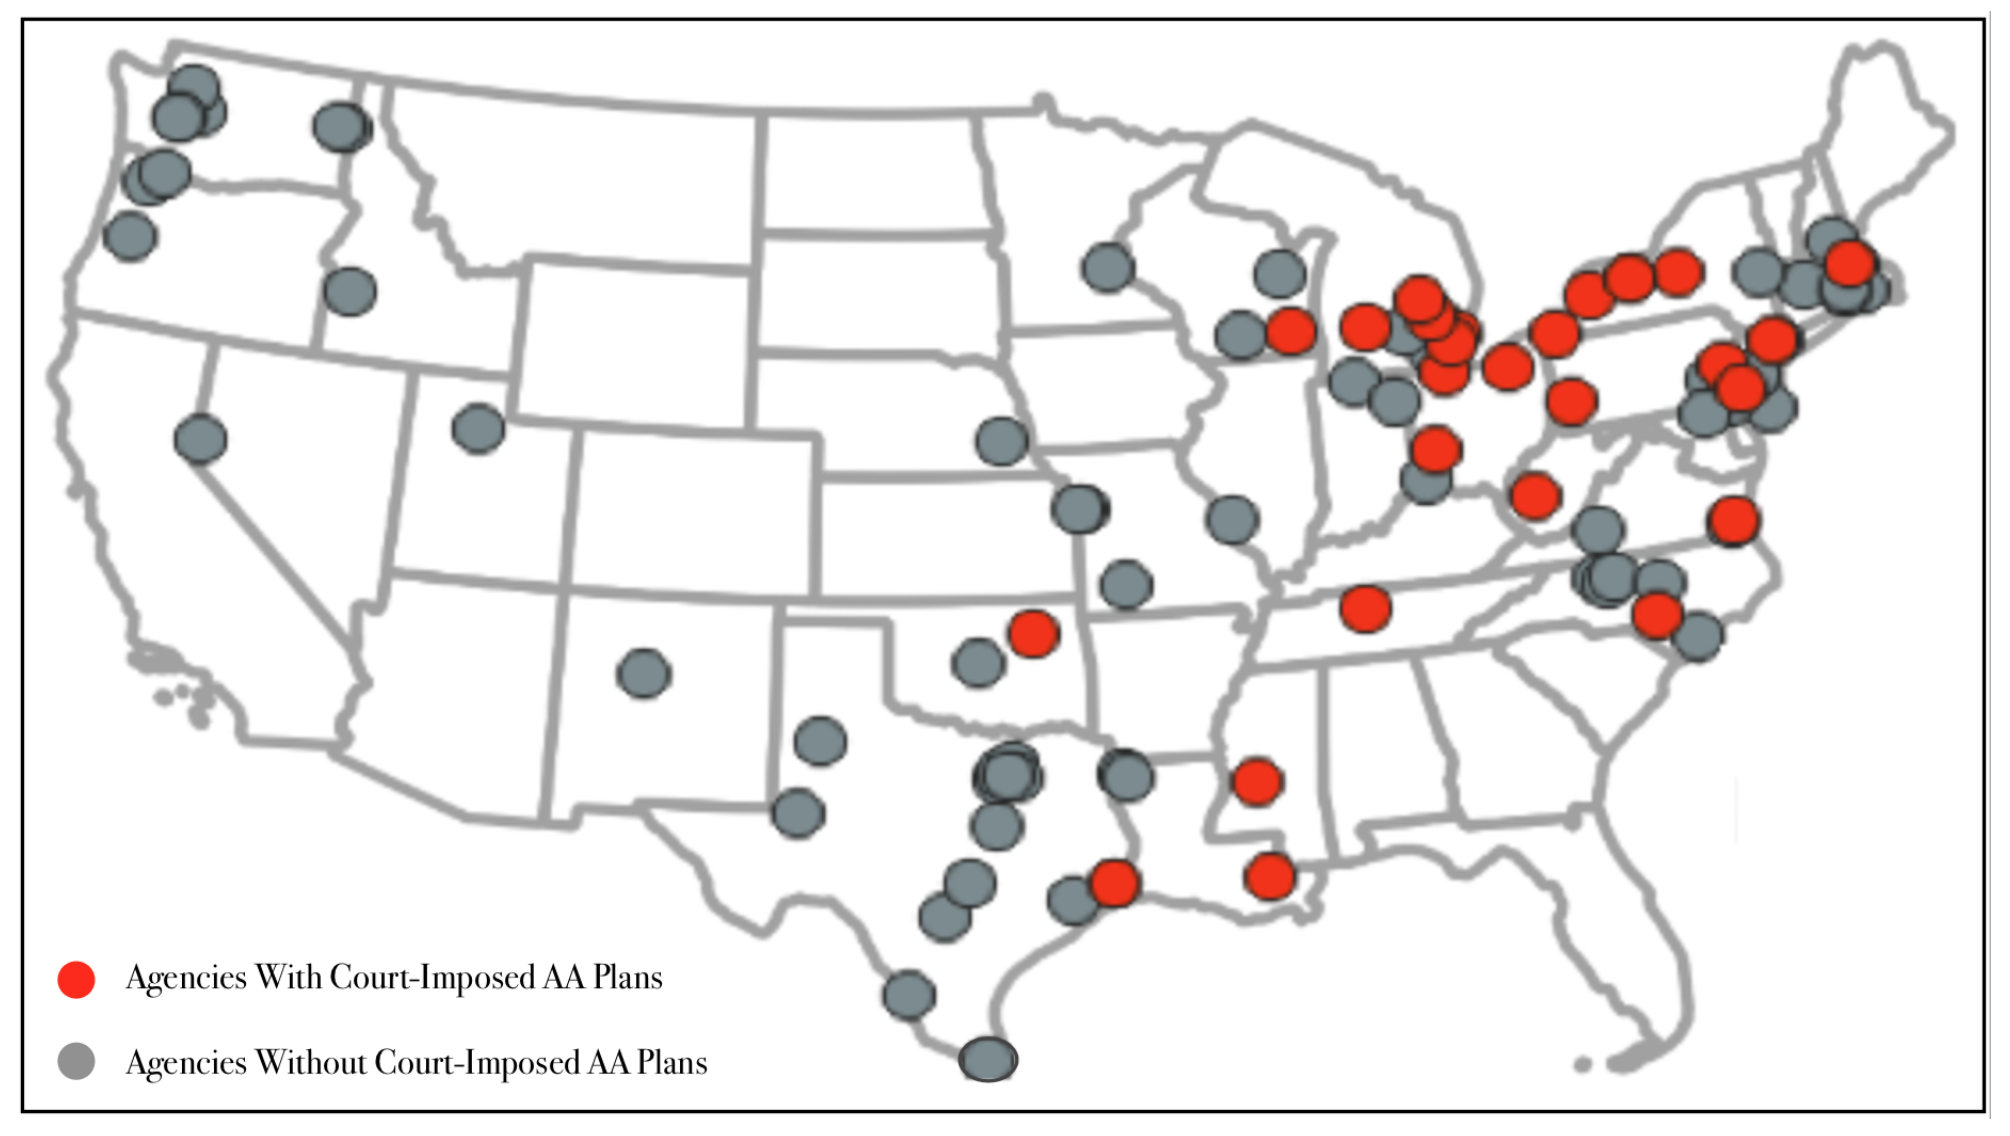
\includegraphics[width=0.78\linewidth]{AAFigures/map.png}
\caption{\textbf{Location of Treated and Untreated Agencies}}
\label{fig:map}
\end{figure}

Write a table directly into the main document. See Table \ref{tab:aa_desc}.
\begin{table}[!htbp] \centering
\caption{\textbf{Summary Statistics, Offense, and Arrest Rates}}
\label{tab:aa_desc}
\begin{threeparttable}
\begin{tabulary}{.5\linewidth}{lccc}
\hline
\hline \
& \textbf{All Agencies} & \textbf{Treated Years} & \textbf{Untreated Years} \\
\hline \\
ln(Violent Offenses Per 100,000) & 6.13 & 6.70 & 6.03 \\
& (1.00) & (0.72) & (1.00) \\
Violent Crime Arrest Rate & 0.51 & 0.44 & 0.52 \\
& (0.34) & (0.15) & (0.36) \\
ln(Property Offenses Per 100,000) & 8.48 & 8.66 & 8.45 \\
& (0.57) & (0.48) & (0.58) \\
Property Crime Arrest Rate & 0.18 & 0.18 & 0.18 \\
& (0.08) & (0.10) & (0.08) \\
Number of Observations & 4,752 & 722 & 4,030 \\
\hline
\end{tabulary}
\begin{tablenotes}
\scriptsize{Table \ref{tab:aa_desc} reports the means for each annual per capita offense/arrest rate variable from 1964 to 2011. \textit{Treated Years} reports means for agencies that had court-imposed AA plans during that year. \textit{Untreated Years} reports means for agencies that did not have court-imposed AA plans during that year. Standard deviations in parentheses.}
\end{tablenotes}
\end{threeparttable}
\end{table}

\subsection{Models and Results}

\subsubsection{Two-way Fixed Effect Difference-in-Differences Models}

\textcolor{green}{How to cite equations. See Equation \ref{eq:2wfe}:}

\begin{equation} \label{eq:2wfe}
    OffenseRates/ArrestRates_{it} = \beta_{0} + \beta_{1}Treat_{it} + \theta_{t} + \alpha_{i} + \epsilon_{it},
\end{equation}

\noindent where $Treat$ is a binary variable equal to one when a unit is subject to a court-imposed affirmative action plan and equal to zero otherwise; $\theta_{t}$ is a time vector containing indicators for the 48 years from 1964 to 2011; and $\alpha_{i}$ is a unit vector containing indicators for the 99 agencies. Standard errors are clustered by agency. The average treatment effect on the treated (ATT) is given by $\beta_{1}$. We estimate the ATT of externally-imposed affirmative action on logged violent and property crime rates per capita and on violent and property crime arrest rates between 1964 and 2011.

\subsubsection{Results for DD Models}

\textcolor{green}{Example of putting sub figures into one. See Figure \ref{fig:hist}.}
\begin{figure}[!h]
\centering
\subfigure{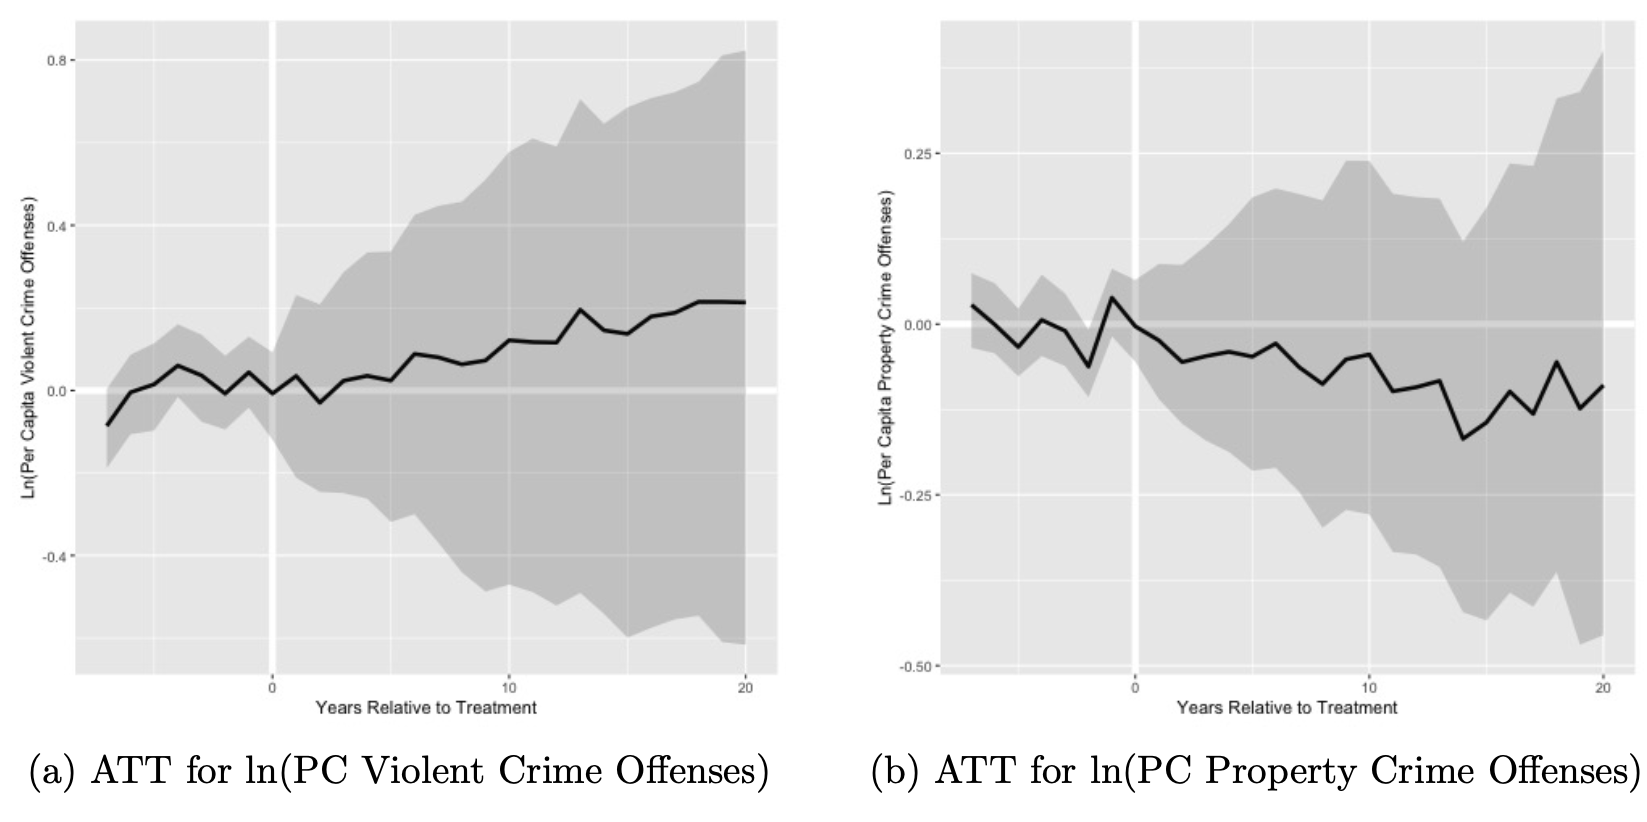
\includegraphics[width=0.75\linewidth]{AAFigures/gsynth1.png}}
\subfigure{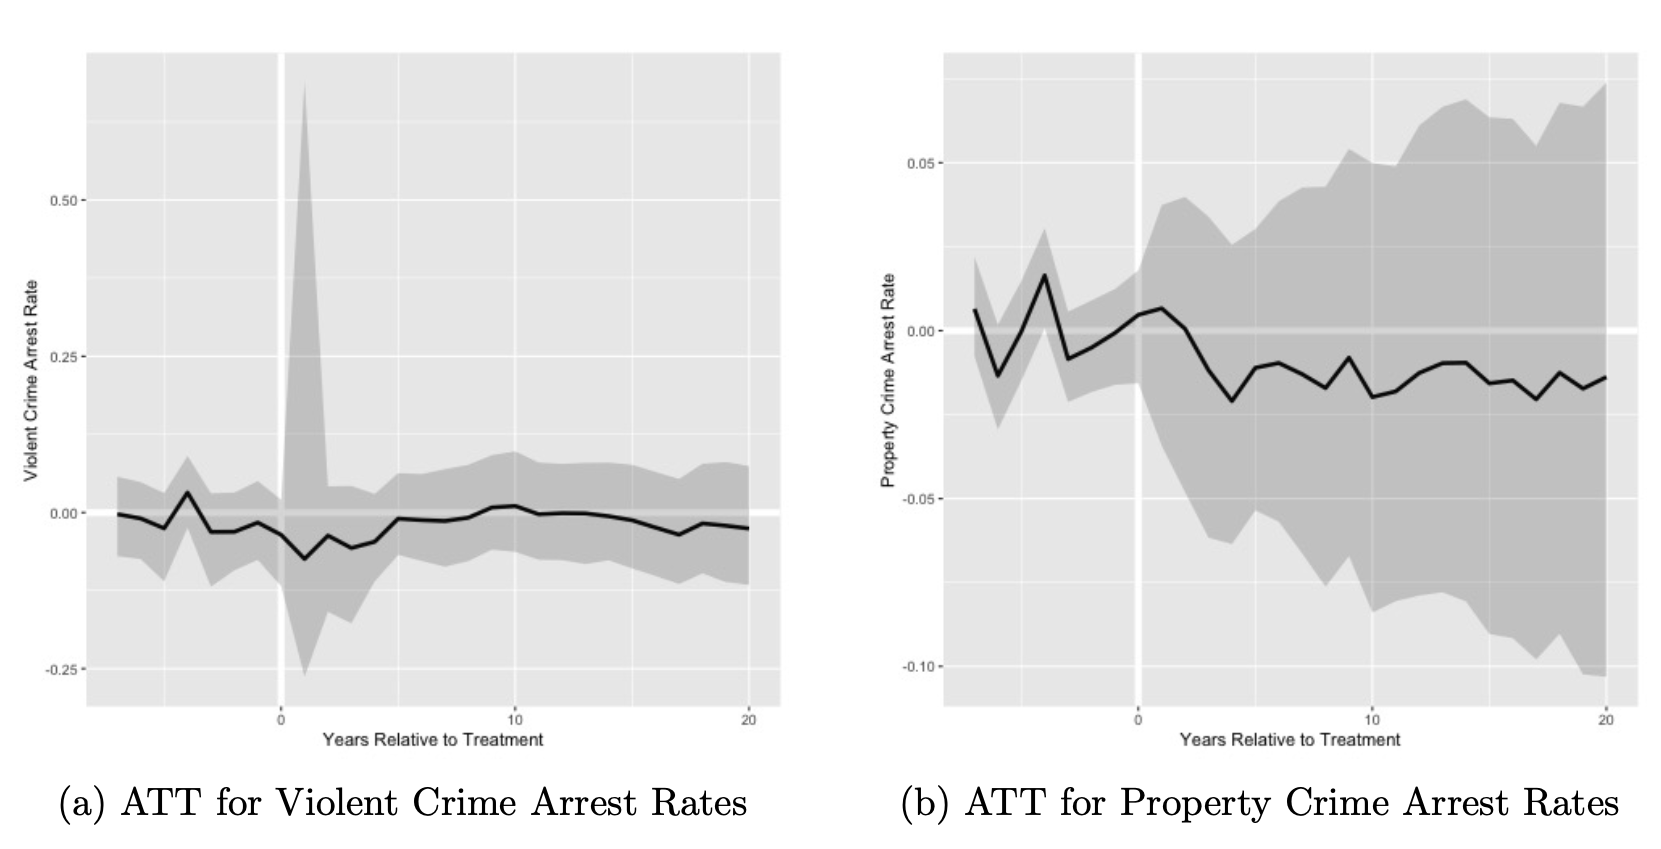
\includegraphics[width=0.75\linewidth]{AAFigures/gsynth2.png}}
\caption{\textbf{Treatment Effects for GSC Models}}
\label{fig:hist}
\end{figure}

\subsection{SUTVA Violation Test}

\textcolor{green}{Example of putting several lines in equation. See Equation \ref{eq:several}.}
\begin{equation} \label{eq:several}
\begin{split}
OffenseRates/ArrestRates_{it} = \beta_{0} + \beta_{1}AATotal_{t} + \beta_{2}(AATotal*EverLitigated)_{it} + \\ + \sum_{p=1}^{P}\xi_{p}t^{p} + \alpha_{i} + \lambda_{i}t + \epsilon_{it},
\end{split}
\end{equation}

\subsection{Conclusion}

\newpage

%%%%% CHAPTER 2 %%%%%%%%%%%

\setcounter{table}{0}
\setcounter{figure}{0}
\setcounter{footnote}{0}
\setcounter{equation}{0}

\section{Chapter 2: Is Police Training an Effective Intervention for Addressing Disparities?}

\textit{Coauthored with [Names of coautohrs]}

\subsection{Introduction}
\textcolor{green}{Example of citing several papers} \citep{wheller13, graziano14, skogan14, thompson16} ...

\subsection{Data \& Background}

\subsubsection{Texas Highway Patrol Data}
\textcolor{green}{Example of putting table by importing a file. See Table \ref{tab:desc_stats_officer}.}
\begin{table}
\centering 
\caption{\textbf{Officer Cohort Descriptive Statistics}}
\label{tab:desc_stats_officer} 
\scalebox{0.565}{
\begin{tabular}{@{\extracolsep{5pt}}lccccccccccccc}
\hline
\hline \
&\multicolumn{1}{c}{\textbf{Overall}}&\multicolumn{1}{c}{\textbf{2007}}&\multicolumn{1}{c}{\textbf{2008}}&\multicolumn{1}{c}{\textbf{2009}}&\multicolumn{1}{c}{\textbf{2010}}&\multicolumn{1}{c}{\textbf{2011}}&\multicolumn{1}{c}{\textbf{2012}}&\multicolumn{1}{c}{\textbf{2013}}&\multicolumn{1}{c}{\textbf{2014}}&\multicolumn{1}{c}{\textbf{2015}}&\multicolumn{1}{c}{\textbf{2016}}&\multicolumn{1}{c}{\textbf{2017}}&\multicolumn{1}{c}{\textbf{2018}}\\
\midrule
Number of Officers         &        2,274&         312&         166&         133&         136&          76&         128&         181&         196&         211&         393&         273&          69\\
\midrule
\textit{1st CD Outside Sample; $>$1st CD w/in} \\
\ \ \ Total         &         107&          26&          14&          12&          17&           2&           6&           8&           5&          14&           3&           3&          0\\
\ \ \ First CD at Academy&           0&           0&           0&           0&           0&           0&           0&           0&           0&           0&           0&           0&            0\\
\ \ \ First CD w/in 0-2 Years&          19&           3&           2&           0&           1&           0&           0&           0&           0&          10&           3&           3&            0\\
\ \ \ First CD w/in 2-4 Years&          30&           0&           0&           1&          13&           0&           1&           6&           5&           4&           0&           0&            0\\
\ \ \ First CD w/in 4-6 Years&          32&          14&           9&           0&           0&           2&           5&           2&           0&           0&           0&           0&            0\\
\midrule 
\textit{1st CD Outside Sample; No CD w/in} \\
\ \ \ Total         &         804&         276&         148&         119&          30&          16&          23&          21&          20&          45&          38&          57&          11\\
\ \ \ First CD at Academy&         355&         173&         108&          54&           0&           0&           1&           2&           0&           7&           4&           5&           1\\
\ \ \ First CD w/in 0-2 Years&         385&          98&          40&          65&          14&           3&           8&          10&          13&          38&          34&          52&          10\\
\ \ \ First CD w/in 2-4 Years&          12&           1&           0&           0&           1&           2&           2&           0&           6&           0&           0&           0&           0\\
\ \ \ First CD w/in 4-6 Years&          33&           2&           0&           0&           1&           8&          12&           9&           1&           0&           0&           0&           0\\
\midrule 
\textit{1st CD w/in Sample} \\
\ \ \ Total         &         696&           3&           4&           2&          77&          53&          91&         139&         123&          93&          92&          19&0\\
\ \ \ First CD at Academy&           0&           0&           0&           0&           0&           0&           0&           0&           0&           0&           0&           0&0\\
\ \ \ First CD w/in 0-2 Years&         132&           0&           0&           0&           1&           1&           4&           0&           6&          29&          72&          19&0\\
\ \ \ First CD w/in 2-4 Years&         294&           0&           0&           0&           6&           5&           8&          77&         114&          64&          20&           0&0\\
\ \ \ First CD w/in 4-6 Years&         192&           0&           0&           0&          11&          37&          79&          62&           3&           0&           0&           0&0\\
\midrule 
\textit{No CD Yet} \\
\ \ \ Total         &         667&           7&           7&           7&          12&           5&           8&          13&          48&          59&         260&         197&          58\\
\ \ \ First CD at Academy&           0&           0&           0&           0&           0&           0&           0&           0&           0&           0&           0&           0&           0\\
\ \ \ First CD w/in 0-2 Years&           0&           0&           0&           0&           0&           0&           0&           0&           0&           0&           0&           0&           0\\
\ \ \ First CD w/in 2-4 Years&           0&           0&           0&           0&           0&           0&           0&           0&           0&           0&           0&           0&           0\\
\ \ \ First CD w/in 4-6 Years&           0&           0&           0&           0&           0&           0&           0&           0&           0&           0&           0&           0&           0\\
\hline
\end{tabular}}
\begin{tablenotes}
\scriptsize{Table \ref{tab:desc_stats_officer} presents descriptive statistics for officer cohorts. Officers are separated by when they took their first Cultural \newline Diversity (CD) training. For officers who have had at least one Cultural Diversity training, results are further \newline disaggregated by whether they received this training at the academy or years after their Basic Peace Officer training.}
\end{tablenotes}
\end{table}

\subsection{Methods \& Results}

\subsubsection{Does Cultural Diversity Training Affect Racial Disparities?}

\subsubsection{Do Other Trainings Affect Racial Disparities?}

\subsubsection{Does Training Affect Outcomes for White Motorists?}

\newpage

%%%%% CHAPTER 3 %%%%%

\setcounter{table}{0}
\setcounter{figure}{0}
\setcounter{footnote}{0}
\setcounter{equation}{0}

\section{Chapter 3: Does the Presence of Female and Minority Police Reduce the Use of Force?}

\subsection{Introduction}

\subsection{Data Sources}

\subsection{Identification Strategy \& Results}

\subsubsection{Dispatch and Arrest Protocol}

\subsubsection{Models}
\textcolor{green}{A second example of how to refer to equations. See Equation \eqref{eq:avail}:}
\begin{equation}
\label{eq:avail}
    BlackAvailRate_{c} = \frac{Number\ of\  Available\  Black\  Officers_c}{Number\ of\ Officers\ on\ Shift_c}
\end{equation}

\textcolor{green}{Use of widehat. See Equation \ref{eq:iv}:}
\begin{equation}
\label{eq:iv}
\begin{split}
    ForceUsed_{c} = \beta_{0} + \beta_{1}\widehat{(BlackOfficer)_{c}} + \delta X_{c} + \lambda_{1} (DayOfWeek)_{c} + \\ \lambda_{2} (HourOfDay)_{c} + \lambda_{3} (DivisionYearWeekShift)_{c} + \epsilon_{c},
\end{split}
\end{equation}
where $\widehat{BlackOfficer_{c}}$ represents the fitted values from the first stage. 

\subsubsection{Main Results}

\subsection{Robustness}

\subsection{Conclusion}

%%%%% REFERENCES %%%%%
\newpage
\bibliographystyle{apalike}
\bibliography{bibliography}

\end{document}

